\documentclass[11pt, oneside]{article}   	% use "amsart" instead of "article" for AMSLaTeX format
\usepackage{geometry}                		% See geometry.pdf to learn the layout options. There are lots.
\geometry{letterpaper}                   		% ... or a4paper or a5paper or ... 
%\geometry{landscape}                		% Activate for rotated page geometry
\usepackage[parfill]{parskip}    		% Activate to begin paragraphs with an empty line rather than an indent
\usepackage{graphicx}				% Use pdf, png, jpg, or eps§ with pdflatex; use eps in DVI mode
								% TeX will automatically convert eps --> pdf in pdflatex		
\usepackage{amssymb}
\graphicspath{ {./Images/} }

%SetFonts

%SetFonts


\title{
A Serious Game for Teaching SQL
}
\author{
Amarnath Kakkar \\
\normalsize University of Bath
}
%\date{}							% Activate to display a given date or no date


\begin{document}



\maketitle
%\section{}
%\subsection{}

\newpage
\tableofcontents

\newpage
\section{Project Idea}

Video games or digital games have become a popular source of entertainment for a wide range of age groups. However, there has been an increasing interest in games that are developed for educational purposes, to be used in educational environments, known as 'serious games'. Serious games are developed with the aim of educating and not merely for entertainment. These games are often compared to traditional teaching methods.

Some basic features of games include the ability to unlock new levels, unlock achievements and gain rewards. These features cause games to be; engaging and motivating, because of the excitement of unlocking achievements and gaining rewards, and the desire to simply progress through the game and potentially beating it. Games are also capable of teaching new skills and getting users to re-apply those skills in various scenarios. This makes games great learning environments. However, there is a lack of literature to prove these claims, and so more empirical studies on the matter are required \cite{MetaAnalysis}.

This project aims to develop a serious game to teach the programming language SQL. The reason that a programming language was chosen as the topic of the educational game is follows:

\begin{itemize}
\item Learning programming languages are a core part of Computer Science courses at University. This allows for a wide range of users to evaluate. 
\item There are complexities to a programming language and to the programs that it can create, this can be used to create a defined structure of progression through the game, starting with basic commands and slowly introducing more difficult concepts.
\end{itemize}





\newpage
\section{Requirements}

Intro

\newpage
\section{Project Plan}

The key milestones for this project are:

\begin{enumerate}
  \item \textit{2nd Nov 2018} - Project Proposal Submission
  \item \textit{30th Nov 2018} - Literature \& Technology Survey Submission
  \item \textit{18th Feb 2019} - Demonstration of Progress
  \item \textit{7th May 2019} - Dissertation Submission
\end{enumerate}

\hfill

The following Gantt Chart (Figure 1) shows the timeline of the proposed work, including the duration and sequences of all main tasks, subtasks and the key milestones listed above.



\begin{figure}[h!]
  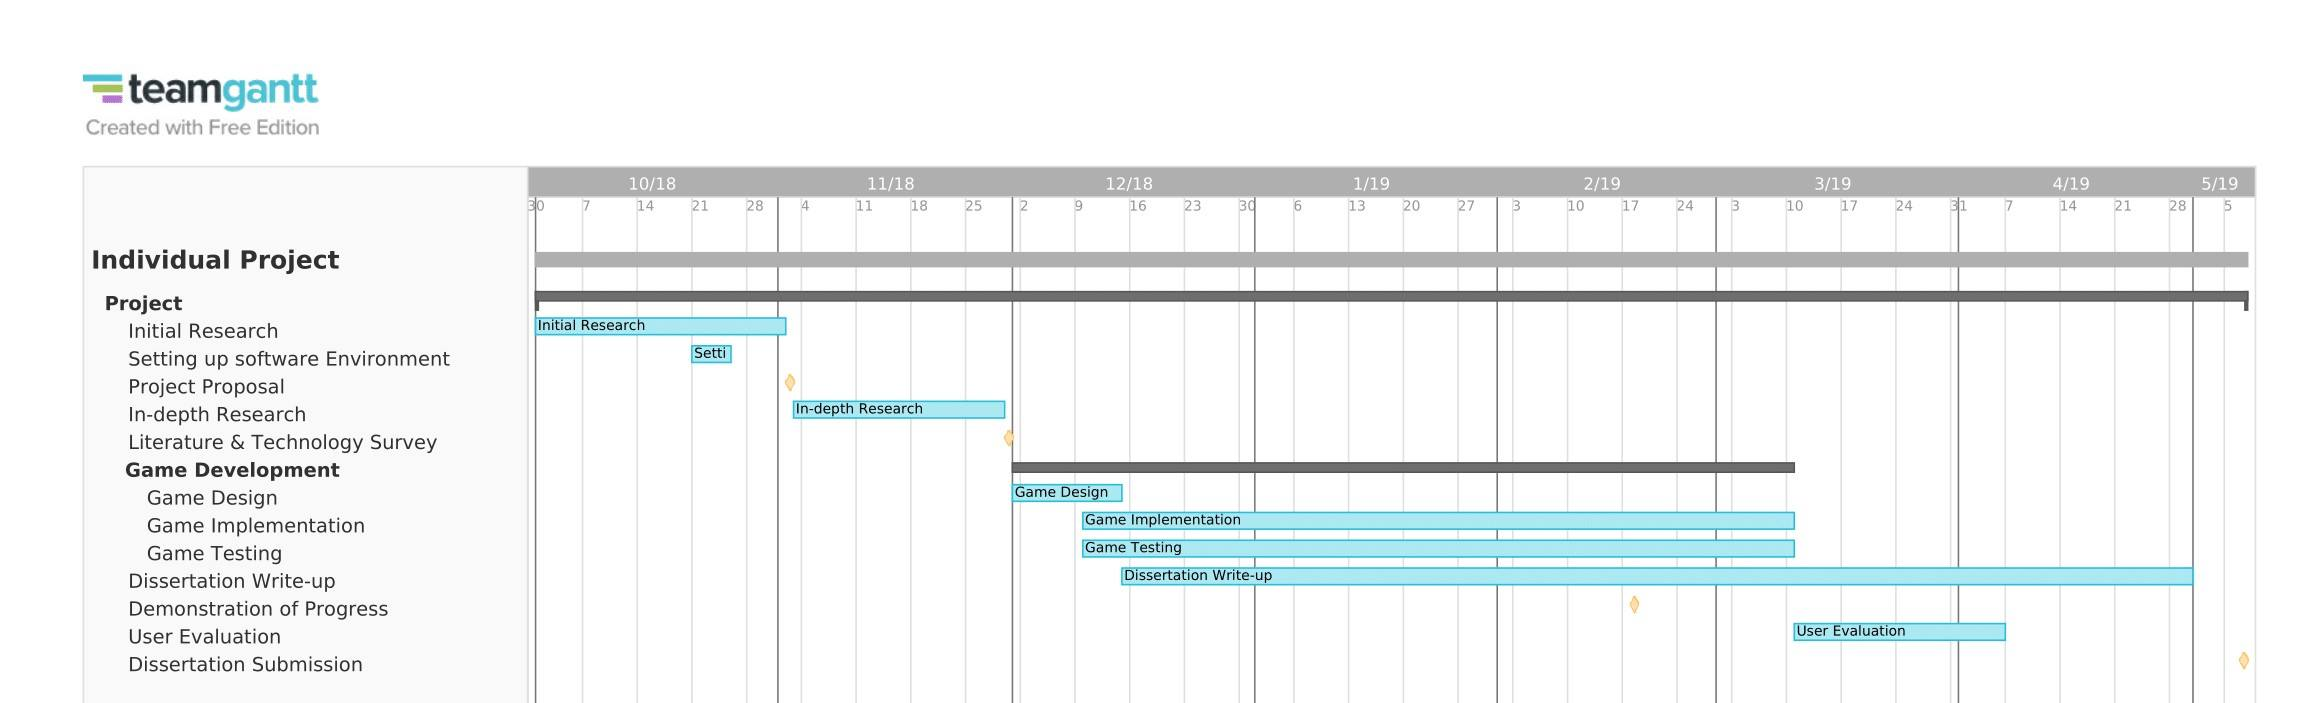
\includegraphics[width=15cm]{GanttChart}
  \caption{Gantt Chart showing the proposed timeline of entire project}
\end{figure}

\newpage
\section{Resource Requirements}

These are some requirements that may be needed to complete this project:

\begin{itemize}
\item Version control software
\item 
\end{itemize}

\newpage
\bibliography{ProposalReferences}
\bibliographystyle{plain}
\end{document}  